\documentclass[12pt]{article}
\usepackage{geometry,float}
\usepackage{amssymb}
\usepackage{amstext,enumerate}
\usepackage{amsmath,amssymb,amsthm,textcomp}
\usepackage{enumitem}
\usepackage{bm}
\usepackage{graphics}
\usepackage{graphicx}
\usepackage{amsthm}
\usepackage{amsmath}
\usepackage{latexsym}
\usepackage{rotate}
\usepackage{lscape}
\usepackage{color}
\usepackage{epsfig,epsf,psfrag}
\usepackage{sectsty}
%\usepackage{natbib}
\usepackage{graphics}
\usepackage{epsfig}
%\usepackage{html} %
%\usepackage{rotate}
\usepackage{multirow}
%\usepackage{lscape}
\usepackage{graphicx}
\usepackage{amsmath}
\usepackage{url}
\usepackage{amsthm}
\usepackage{amssymb}
\usepackage{sectsty}
\usepackage{epsfig,natbib}
%\usepackage{slashbox} %
%\usepackage[authoryear,super]{natbib}
%\usepackage[mathscr]{eucal}
\usepackage{rotate}
\usepackage{lscape}
\usepackage{setspace}
\usepackage{subcaption}
\usepackage{float}
\usepackage{graphicx}
\usepackage{mathtools}
%\usepackage{enumitem}
\newtheorem{Theorem}{Theorem}%[section]
\newtheorem{Lemma}{Lemma}
\newtheorem{Corollary}{Corollary}
\include{mathdefn2}

%\bibliographystyle{asa}
%\def\references{\bibliography{array,mds,tree,C:/hanstex/macros/bib/4-1-10}}
\def\red{\textcolor{red}}
\def\blue{\textcolor{blue}}

\renewcommand\thesection{\arabic{section}.}
\renewcommand{\thesubsection}{\thesection\arabic{subsection}}
\sectionfont{\centering\bf\sf\normalsize}
\subsectionfont{\sf\normalsize}
\newcommand{\sups}{\sup_{s \in \mathcal{S}}}
\newcommand{\lN}{t_l}
\newcommand{\suml}{\sum_{l=1}^{N}}
\setlength{\textheight}{8.5in} \setlength{\textwidth}{6.3in}
\setlength{\topmargin}{0.2in} \setlength{\oddsidemargin}{0.1in}
\setlength{\evensidemargin}{0.12in} \tolerance=500
\newcommand{\Appendix}{\appendix
\def\thesection{A.\arabic{section}}
\def\thesubsection{\Alph{section}.\arabic{subsection}}}


\hoffset 0in \marginparsep 0in \marginparwidth 0in

\voffset 0in %-0.3in
\headsep 0in %0.5
\footskip 28pt

\setlength{\baselineskip}{22pt} \setlength{\parskip}{0.0in}
\renewcommand\refname{\centerline{\bf \sf REFERENCES}}
\renewcommand{\baselinestretch}{1.6} %{2} %{1.4}
\renewcommand{\arraystretch}{1.0} %{1.2}
\newcommand{\single}{\renewcommand{\baselinestretch}{1.2}\normalsize}
\newcommand{\double}{\renewcommand{\baselinestretch}{1.63}\normalsize}

  %reduce spacing between bibitems with natbib package
  \let\oldthebibliography=\thebibliography
  \let\endoldthebibliography=\endthebibliography
  \renewenvironment{thebibliography}[1]{
    \begin{oldthebibliography}{#1}
      \setlength{\parskip}{0ex}
      \setlength{\itemsep}{0ex}
  }
  {
    \end{oldthebibliography}
  }

\newcommand{\bea}{\begin{eqnarray*}}
\newcommand{\eea}{\end{eqnarray*}}
\newcommand{\be}{\begin{eqnarray}}
\newcommand{\ee}{\end{eqnarray}}
\newcommand{\ed}{\end{document}}
\newcommand{\et}{\textit{et al. }}
\newcommand{\btab}{\begin{tabular}}
\newcommand{\etab}{\end{tabular}}
\newcommand{\np}{\newpage}
\newcommand{\la}{\label}
\newcommand{\bi}{\begin{itemize}}
\newcommand{\ei}{\end{itemize}}
\newcommand{\bfi}{\begin{figure}}
\newcommand{\efi}{\end{figure}}
\newcommand{\ben}{\begin{enumerate}}
\newcommand{\een}{\end{enumerate}}
\newcommand{\bay}{\begin{array}}
\newcommand{\eay}{\end{array}}
\newcommand{\bs}{\boldsymbol}
\newcommand{\mb}{\boldsymbol}
\newcommand{\nn}{\nonumber}
\newcommand{\rs}{\vspace{-.2cm}}

\def\vsp{\vspace{0.3cm}}
\def\vs{\vspace{.5cm}}

\def\bb{\color{blue}}
\def\eb{\color{black}}

\def\bco{\iffalse}
\def\cov{{\rm cov}}
\def\var{{\rm var}}
\def\corr{{\rm corr}}
\def\diag{{\rm diag}}
\def\trace{{\rm trace}}
\def\logit{\hbox{logit}}
\def\expit{\hbox{expit}}
\def\ci{\cite}
\def\cp{\citep}
\def\eps{\varepsilon}
\def\rs{\vspace{-.1in}}
\def\DReg{\emph{Dense Regular Design}}
\def\reg{\emph{Regular Design}}
\def\ran{\emph{Random Design}}
\def\DRan{\emph{Dense Random Design}}
\def\Sparse{\emph{Sparse Random Design in $s$}}
\def\DEST{\emph{empirical estimators}}
\def\SEST{\emph{smoothing estimators}}
\newcommand{\no}{\noindent}
\newcommand{\bc}{\begin{center}}
\newcommand{\ec}{\end{center}}
\newcommand{\Ahat}{\frac{1}{\hat{\lambda}_k}}
\newcommand{\A}{\frac{1}{\lambda_k}}
\newcommand{\Bhat}{\hat{G}^{(1,0)}(t,s)}
\newcommand{\B}{G^{(1,0)}(t,s)}
\newcommand{\Chat}{\hat{\phi}_k(s)}
\newcommand{\C}{\phi_k(s)}
\newcommand{\hsig}{h_{\mu,1}^2\gamma_{\kappa_1}^2}
\newcommand{\hgam}{h_{G,1}^2\gamma_1^2}
\newcommand{\hgamm}{h_{G,1}^2\gamma_2^2}
\newcommand{\supmu}{\sup_{t\in\mathcal{T}}}
\newcommand{\supG}{\sup_{t,s\in\mathcal{T}}}
\newcommand{\xkhat}{\hat{X}'_{i,K}(t)}
\newcommand{\xktilde}{\widetilde{X}'_{i,K}(t)}
\newcommand{\xtilde}{\widetilde{X}'_i(t)}
\newcommand{\tbeta}[1]{\tilde{\beta}_{#1}}
\newcommand{\tG}{\widetilde{G}_i(T_{ij},T_{il})}
\newcommand{\dbsum}{\sum_{i=1}^n \frac{1}{EN(EN-1)}\sum_{1\leq j\neq l\leq N_i}}
\newcommand{\superscript}[1]{\ensuremath{^\textrm{#1}}}
\newcommand{\subscript}[1]{\ensuremath{_\textrm{#1}}}
\newcommand{\mybm}[1]{\mbox{\boldmath$#1$}}
\newcommand{\sigYinv}{\mbox{\boldmath$\Sigma$}_{\tiny{\mathbf{Y}_i}}^{\tiny{-1}}}
\newcommand{\sigYinvh}{\hat{\mbox{\boldmath$\Sigma$}}_{\tiny{\mathbf{Y}_i}}^{\tiny{-1}}}
\newcommand{\sigY}{\mbox{\boldmath$\Sigma$}_{\tiny{\mathbf{Y}_i}}}
\newcommand{\sigYh}{\hat{\mbox{\boldmath$\Sigma$}}_{\tiny{\mathbf{Y}_i}}}
\newcommand{\mt}{\mathcal{T}}
\newtheorem{thm}{Theorem}
\newcommand{\ms}{\mathcal{S}}
\newcommand{\Var}{\text{Var}}
\newcommand{\Cov}{\text{Cov}}
\DeclareMathOperator*{\argmax}{argmax}
\DeclareMathOperator*{\argmin}{argmin}
\def\foot#1#2{{\baselineskip=9pt\sevenrm\footnote{$^{#1}$}{#2}}}
\def\nh{\noindent\hangindent=1.5truecm\hangafter=1}


\newcommand{\sm}{}
\bibpunct{(}{)}{;}{a}{}{,}

\begin{document}
\thispagestyle{empty} \single \bc {\bf \sc \Large Tree Cover Variability Increases from 2005 to 2100
in Sub-Saharan Africa}
%$^{\dagger *}$}
\vspace{0.15in}\\
Eric Kalosa-Kenyon, Cody Carroll, and Amy Kim \\
 Department of Statistics, University of California, Davis \\
 \ec \centerline{December 2017}

%\vspace{0.1in} \thispagestyle{empty}
%\bc{\bf \sf ABSTRACT} \ec \vspace{-.1in} \no 
%\setstretch{1}


%
%\no {KEY WORDS:\quad Functional data analysis, accelerated longitudinal study, autonomous differential equation, uniform convergence, monotonic process, nonparametric estimation, hippocampal volume}.
%\thispagestyle{empty} \vfill
%\noindent \vspace{-.2cm}\rule{\textwidth}{0.5pt}\\
%{\small Matthew Dawson is  Graduate Student Researcher and Hans-Georg M\"uller is Professor at the Department of Statistics, University of California, Davis. 
%This research was  supported by NSF grants DMS-1228369 and
%DMS-1407852. The data used in this paper are from the Alzheimer's Disease Center at University of California Davis, supported by NIH and NIA grant P30 AG10129.
%We are grateful to the Editor, an Associate Editor and two referees for
%constructive critiques, which led to many improvements in the
%paper. Special thanks are due to  Wenwen Tao and Wesley Thompson for discussions of the problem of longitudinal snippet data.}

\newpage
\pagenumbering{arabic} \setcounter{page}{1}

\newpage
\pagenumbering{arabic} \setcounter{page}{1} \double

\bc {\bf \sf 1.\quad CHANGEPOINT ANALYSIS }\sm \ec \rs

\no  Instead of dealing with the non-stationarity of our series by differencing and using the ARIMA framework, another approach is to notice that there are specific points in time where the time series changes behavior in one fell swoop. An example of this is around the year 2025, where the series jumps up to a mean level of around 11.75 and stays there. Figure 1 illustrates this "jump" with a red dashed line.
\begin{figure}[h]
	\centering
	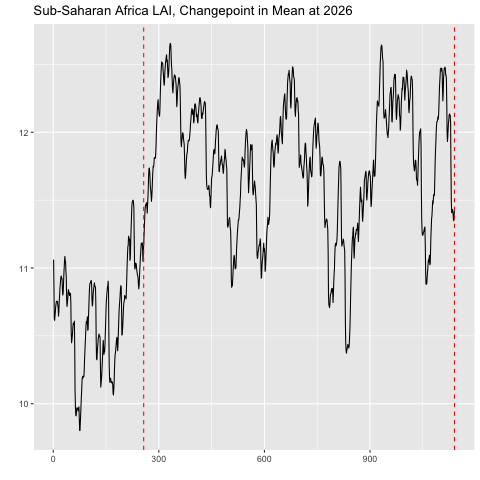
\includegraphics[width=5in, height=4.5in]{../img/changepoint_LAI.png}
	\caption{LAI TS}
\end{figure}

This point in time is called a changepoint. We give a short introduction on changepoint detection methods.\clearpage
\noindent { \sf 1.1. \quad Changepoint Detection} Conceptually, for data $Z_1,...,Z_n$, a changepoint $\tau$ is a point in time, such that $Z_1,...,Z_\tau$ differ from  $Z_\tau+1,...,Z_n$. For the sake of illustration, we take a simple example. Assume the parametric form
\begin{equation*}
	Z_t|\theta_t\sim N(\theta_t,1) \tag*{where $\theta_t=1 ~\text{if}~ t\leq\tau$ and $\theta_t=0 ~\text{if}~ t>\tau$}.
\end{equation*} An example of such a process is depicted in Figure 2.
\begin{figure}[h]
	\centering
	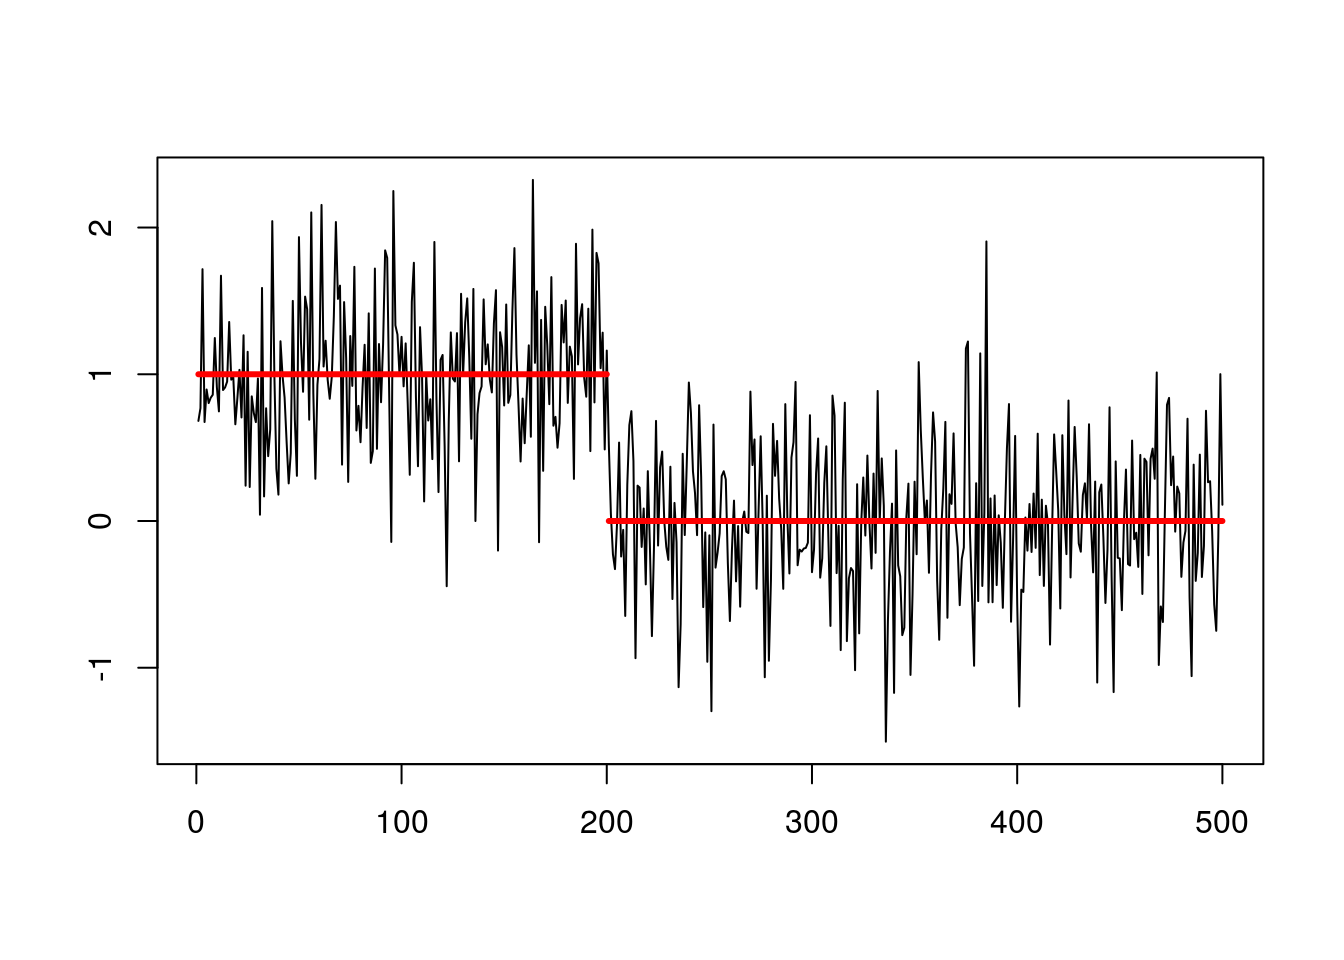
\includegraphics[width=0.75\linewidth]{../img/changepointex.png}
	\caption{Example of a Changepoint}
\end{figure}

It's intuitively clear from the picture that the change occurs at $\tau=200$, but how do we detect where a changepoint occurs, mathematically? One approach is to use a Likelihood Ratio Test. We state the hypotheses as: 
\begin{equation*}
	H_0:\theta_t=\theta~ \forall~ t \quad\text{vs.} \quad H_1:\theta_t=\theta_1,~t\leq\tau;~ \theta_t=\theta_2,~t>\tau 
\end{equation*}
To construct the likelihood ratio statistic, we need to maximize the likelihood under the null and alternative.  We let $p(\cdot)$ be the probability density function associated with the distribution of the data and $\hat{\theta}$ is the maximum likelihood estimate of the parameters. Under $H_0$, the maximum log-likelihood is $\log p(y_{1:n}|\hat{\theta})$.
Under $H_1$ with a changepoint $\tau$, the maximum log-likelihood is $ML(\tau) = \log p(y_{1:\tau}|\hat{\theta}_1) +  \log p(y_{\tau+1:n}|\hat{\theta}_2)$. Therefore the likelihood ratio statistic is:
\begin{equation*}
	\Lambda(\tau)=\dfrac{\max_\tau ML(\tau)}{\log p(y_{1:n}|\hat{\theta})}
\end{equation*}
A more commonly used version of this statistic is the log-LR statistic:
\begin{equation*}
2\log\Lambda(\tau)=2\left[\max_\tau ML(\tau)-\log p(y_{1:n}|\hat{\theta})\right]\
\end{equation*}
We compare this statistic with a cut-off value, $\lambda$. If $LR>\lambda$, then we reject $H_0$ and estimate the changepoint as 
\begin{equation*}
\hat{\tau}=\arg\max_\tau LR(\tau)
\end{equation*}
There are many different ways to select $\lambda$. Selecting an optimal value of $\lambda$ remains an open research topic in changepoint analysis. We use the package 'changepoint' to investigate if our LAI time series has a changepoint, using a specific $\lambda$ value that takes into consideration the inherent correlation between observations of a time series.




\ed
